\documentclass[a4paper,10pt]{report}
\usepackage[T1]{fontenc}
\usepackage{mathptmx}
\usepackage{graphicx}
\graphicspath{ {Diagrams/} }

\title{Assignment 1.2 documentation}

\author{Péter Zaváczki\\30433}

\begin{document}

\maketitle

\section{Requirements}
Design implement and test a three-tiered distributed system to view and create flights for an airport.
The system consists of the following tiers: Presentation, Business Layer and Data Access.

\section{Functional requirements}
\begin{itemize}
    \item Users log in. Users are redirected to the page corresponding to their role. 
    \item Client role
    \begin{itemize}
        \item A client can view on his/her page all the flights in a list or table.
        \item A client can query for the local time of the flight arrival and departure cities computed based on cities geographical coordinates. 
    \end{itemize}
    \item Administrator role
    \begin{itemize}
        \item The administrator can perform CRUD operations on flights (Create, Read, Update and Delete) 
    \end{itemize}
    \item Each flight consists of the following information: flight number, airplane type, departure city, departure date and hour, arrival city, arrival date and hour. 
    \item Each city has associated its geographical coordinates: latitude and longitude.
    \item In order to display the local time, the geographical coordinates of the city are passed to an external web service which will return the actual time value. 
    \item The simple users will not be able to enter the administrator page (e.g. by log-in and then copy-paste the admin URL to the browser)
\end{itemize}

\section{Non-functional requirements}
\begin{itemize}
    \item Security: use authentication in order to restrict users to access the administrator pages
\end{itemize}

\section{Implementation technologies}
\begin{itemize}
    \item HTML
    \item Java servlets
    \item Hibernate ORM
\end{itemize}

\section{Conceptual architecture}
This application has a Client-Server architecture, the Client being represented by the user's webbrowser, and the server, which can serbe multiple clients simultaneously.
On the server we can find a three tier structure.

The data access layer being implemented with Data Access Object classes, using the Hibernate Framework for ORM. 

The business layer uses the command design pattern for every action a user can perform.
These commands are then used in the servlets, which serve as the backbone of our webapp.
The servlets communicate with the client with the help of HTTP requests.

The presentation layer is composed of the user interface provided by the HTML files, which are loaded by the client's browser.
This can be seen on figure \ref{fig:architecture_diagram}.

\begin{figure}[h]
    \centering
    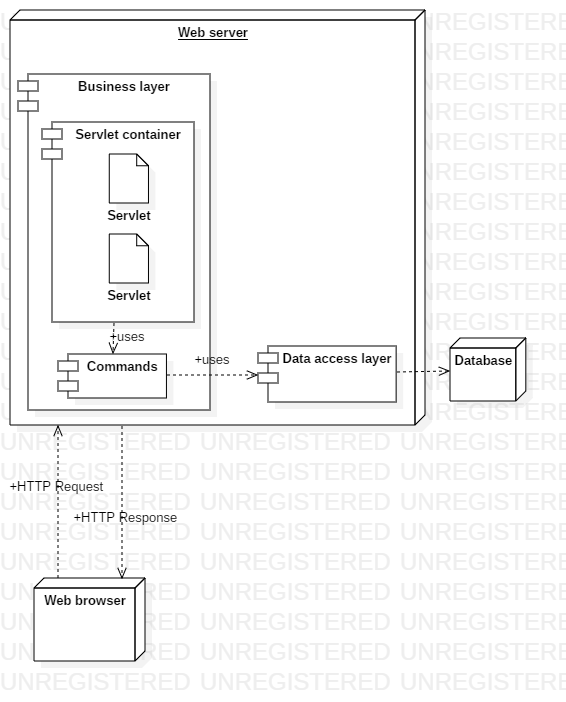
\includegraphics[width=1\textwidth]{architecture_diagram.png}
    \caption{The conceptual architecture diagram of the project}
    \label{fig:architecture_diagram}
\end{figure}

\section{Database}
The database contains three tables.
The \textit{users} table contains data about the users: their username, password, both of type varchar(255) and admin status of type int(11), 1 meaning that the user is an admin and 0 meaning that it is a regular user.
The \textit{cities} table contains data about the cities the planes can fly to and from: the city name, of type varchar(255), its latitude and its logitude, both in float.
The \textit{flights} table contains data about the flights: the flight number, of type int, the airplane type of type varchar(255), and the data pair about the departures and arrivals, the city is represented by an int, the id of the city from the \textit{cities} table, and a varchar(255) field for storing the times.
This structure can be seen on figure \ref{fig:database_diagram}.

\begin{figure}[h]
    \centering
    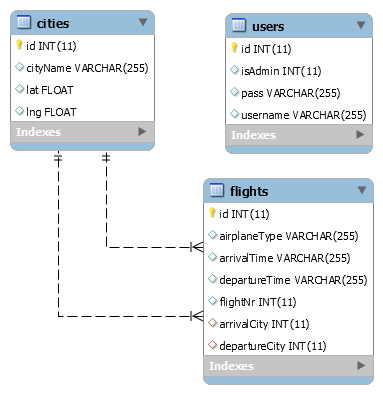
\includegraphics[width=0.75\textwidth]{database_diagram.png}
    \caption{The diagram of the database of the project}
    \label{fig:database_diagram}
\end{figure}

\section{Deployment}
The webapp is deployed on multiple nodes.
The database is on the database server, which hosts a MySql database.
The Webserver contains the Web Application Resource (WAR) files.
The Client has a web browser, on which the HTML presentation files are loaded.
This deployment can be seen on figure \ref{fig:deployment_diagram}.

\begin{figure}[h]
    \centering
    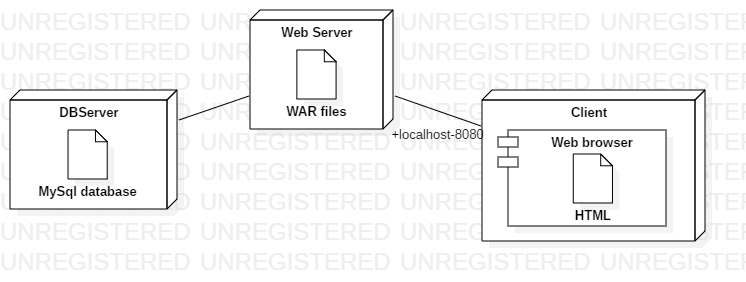
\includegraphics[width=1\textwidth]{deployment_diagram.png}
    \caption{The deployment diagram of the project}
    \label{fig:deployment_diagram}
\end{figure}

\section{Build considerations}
\begin{itemize}
    \item The application differentiates between the user types using a field in the database called isAdmin.
    Users are redirected to their corresponding pages based on their isAdmin fields.
    \item The application uses cookies to ensure that the users get back to the correct page after closing the flight list (admins to the admin page etc.)
    \item When displaying the flight table, we generate the HTML code from the servlets, when we are dealing with static pages, we redirect the user to a pre-written HTML page.
\end{itemize}


\end{document}
